\documentclass[12pt]{article}

% Load packages
\usepackage{cite}              % Make references as [1-4], not [1,2,3,4]
\usepackage{url}              	% Formatting web addresses
\usepackage{ifthen}           	% Conditional
\usepackage{multicol}			% Multi-column pages
\usepackage[utf8]{inputenc}   	% Unicode support
\usepackage{amsmath}           % Support for writing math formulas
\usepackage{amssymb}           % Support for writing math formulas
\usepackage{epsfig}            % Support separate PostScript files for figs
\usepackage{epstopdf}			% Converts eps figs to pdf
\usepackage{graphicx}			% Graphics functions
\usepackage[margin=0.1pt,font=footnotesize,labelfont=bf]{caption}
% \usepackage{caption}			% Styles figure captions
\usepackage{setspace}			% Provides line spacing environments
\usepackage{colortbl}
\usepackage[wide]{sidecap}		% Can typeset caption aside the figure, allows use of margin for figs wider than \textwidth.
\usepackage[square,sort,comma,numbers]{natbib}
% \usepackage[authoryear,square,comma,sort&compress]{natbib}
\usepackage{supertabular}		% Tables spanning multiple pages
\usepackage{comment}
\usepackage{lineno}
\urlstyle{rm}					% URL style
\usepackage{wrapfig}			% Wrap text around figures
\usepackage[FIGTOPCAP,nooneline]{subfigure}
\captionsetup{font={scriptsize},aboveskip=0pt}	% Styles figure captions
\usepackage{simplemargins}
\setallmargins{1.0in}         % Set all margins
% \setlength\bibsep{0pt}     % Single spaced bib
\date{} 
\doublespacing
% \singlespacing
\frenchspacing     % Eliminates double spaces between sentences

\makeatletter
\renewcommand\subsection{\@startsection
	{subsection}{2}{0mm}
	{-0.05in}
	{-0.5\baselineskip}
	{\normalfont\normalsize\bfseries}}
\renewcommand\subsubsection{\@startsection
	{subsubsection}{2}{0mm}
	{-0.05in}
	{-0.5\baselineskip}
	{\normalfont\normalsize\itshape}}
\renewcommand\section{\@startsection
	{subsection}{2}{0mm}
	{-0.2in}
	{0.05\baselineskip}
	{\normalfont\large\bfseries}}	
\renewcommand\paragraph{\@startsection
	{paragraph}{2}{0mm}
	{-0.05in}
	{-0.5\baselineskip}
	{\normalfont\normalsize\itshape}}
\makeatother

\newboolean{publ}

%Publication style settings
%\newenvironment{bmcformat}{\fussy\setboolean{publ}{true}}{\fussy}
\renewcommand{\rmdefault}{phv}\renewcommand{\sfdefault}{phv}
\renewcommand{\bibnumfmt}[1]{#1.}    % Change the number format in the ref list
\renewcommand{\figurename}{Fig.}     % Change Figure to Fig.

%%%%%%%%%%%%%%%%%%%%%%%%%%%%%%%%%%%%%%%%%%%%%%%%%%%%%%%%%%%%%%%%%%%%%
%%%%%%%%%%%%%%%%%%%%%%%%%%%%%%%%%%%%%%%%%%%%%%%%%%%%%%%%%%%%%%%%%%%%%

\begin{document}

%%%%%%%%%%%%%%%%%%%%%%%%%%%%%%%%%%%%%%%%%%%%%%%%%%%%%%%%%%%%%%%%%%%%%
% TITLE PAGE
%%%%%%%%%%%%%%%%%%%%%%%%%%%%%%%%%%%%%%%%%%%%%%%%%%%%%%%%%%%%%%%%%%%%%
\begin{titlepage}

{\par\centering\textbf{\Large Improving Glycosylation Efficiency in \textit{Escherichia coli} through Model-Guided Metabolic Engineering}}
\vspace{0.05in}
{\par \centering \large{Joseph A. Wayman$^{1}$, Thomas J. Mansell$^{2}$, Matthew P. DeLisa$^{3}$, and Jeffrey D. Varner$^{4*}$}}
\vspace{0.10in}
{\par \centering \large{$^{1*}$School of Applied and Engineering Physics, Cornell University, Ithaca, NY 14853}}
{\par \centering \large{$^{2*}$School of Chemical and Biological Engineering, Iowa State University, Ames, IA 50011}}
{\par \centering \large{$^{3*}$School of Chemical and Biomolecular Engineering, Cornell University, Ithaca, NY 14853}}
{\par \centering \large{$^{4*}$School of Chemical Engineering, Purdue University, West Lafayette, IN 47907}}
\vspace{0.1in}
{\par \centering \textbf{Running Title:}~Model-guided glycoengineering in \textit{E. coli}}
\vspace{0.1in}
{\par \centering \textbf{To be submitted:}~\emph{Metabolic Engineering}}
\vspace{0.5in}
{\par \centering $^{*}$Corresponding author:}
{\par \centering Jeffrey D. Varner,}
{\par \centering Professor, School of Chemical Engineering,}
{\par \centering Forney Hall, 480 Stadium Mall Drive, Purdue University, West Lafayette, IN 47907} 
{\par \centering Email: jdvarner@purdue.edu}
{\par \centering Phone: (765) 496 - 0544} 
{\par \centering Fax: (765) 494 - 0805} 
\end{titlepage}
\date{}
\thispagestyle{empty}
\pagebreak

%%%%%%%%%%%%%%%%%%%%%%%%%%%%%%%%%%%%%%%%%%%%%%%%%%%%%%%%%%%%%%%%%%%%%
% ABSTRACT
%%%%%%%%%%%%%%%%%%%%%%%%%%%%%%%%%%%%%%%%%%%%%%%%%%%%%%%%%%%%%%%%%%%%%
\section*{Abstract}

Abstract goes here ...

%%%%%%%%%%%%%%%%%%%%%%%%%%%%%%%%%%%%%%%%%%%%%%%%%%%%%%%%%%%%%%%%%%%%%
% INTRODUCTION
%%%%%%%%%%%%%%%%%%%%%%%%%%%%%%%%%%%%%%%%%%%%%%%%%%%%%%%%%%%%%%%%%%%%%
\newpage
\setcounter{page}{1}
\linenumbers
\section*{Introduction}

Asparagine-linked (N-linked) glycosylation is the most common protein modification in eukaryotes, affecting over two-thirds of the proteome. 
N-linked glycans are complex, branched oligosaccharides, assembled on lipid carriers in the endoplasmic reticulum membrane and transferred to specific asparagine residues of acceptor proteins. 
Approximately 70\% of therapeutic proteins require the attachment of complex branches of sugars to specific amino acid residues \cite{2013-merritt-fisher-delisa-BiotechBioeng}. 
This common post-translational modification affects various protein properties including pharmacokinetic activity and immunogenicity \cite{2010-sola-griebenow-Biodrugs}. 
Currently, eukaryotes possessing native glycosylation machinery serve as the preferred production host of therapeutic glycoproteins. 
Eukaryotic production hosts suffer from several limitations including slow growth and a susceptibility to viral and bacterial infection. 
Also, eukaryotes produce a variety of glycan structures and glycosylate proteins with a range of site occupancy, making purification of the desired glycoform difficult \cite{2013-merritt-fisher-delisa-BiotechBioeng}. 
Though once thought only to occur in eukaryotes, protein glycosylation has been discovered in all other domains of life, including bacteria, spurring interest in the development of alternative glycoprotein expression platforms. 
The most well-characterized bacterial glycosylation system is that of the human pathogen \textit{Campylobacter jejuni} \cite{1999-szymanski-guerry-MolMicrob}. 
The \textit{C. jejuni} glycan has the form of a branched heptasaccharide Glc$\,$GalNAc$_5$$\,$Bac, where Glc is glucose, GalNAc is N-acetylgalactosamine, and Bac is bacillosamine. 
This glycan is assembled on the lipid carrier undecaprenyl pyrophosphate (UDCP) on the cytoplasmic face of the inner membrane by an enzyme pathway encoded by the \textit{pgl} (protein glycosylation) genetic locus (Fig. \ref{fig-glyco-Ecoli}). 
The fully assembled glycan is flipped across the membrane and transferred to asparagine residues on acceptor proteins by an oligosaccharyltransferase (OST) called PglB. 
PglB attaches the heptasaccharide to periplasm-localized proteins containing the consensus sequence D/E-X-N-X-S/T, where X is any residue except proline \cite{2011-fisher-haitjema-delisa-AppEnvMicrobio}. 
The functional transfer of this system into \textit{E. coli} has spurred interest in producing non-native glycans in a more genetically tractable host \cite{1999-szymanski-guerry-MolMicrob,2002-wacker-aebi-Sci}. 

By now, production of a variety of periplasmic, extracellular, and secretory proteins has been demonstrated in glycosylation-competent \textit{E. coli} \cite{2011-fisher-haitjema-delisa-AppEnvMicrobio}. 
Producing glycoprotein from prokaryotic hosts continues to suffer from several limitations including poor glycosylation efficiency and insufficient yield. 
The highest reported efficiency, percent of acceptor protein glycosylated, using the \textit{C. jejuni} system has been 47\% \cite{2011-pandhal-wright-BiotechBioeng}. 
Synthesis of more complex, highly branched glycan, like those found in humans, has proved challenging. 
Recently, a key step in human-like glycan production was achieved in \textit{E. coli} with the recombinant expression of a synthetic glycosylation pathway able to assemble the tri-mannose core glycan \cite{2012-valderrama-rincon-delisa-NatChemBio}. 
The pathway yielded approximately 50 $\mu$g/L of glycosylated protein with an efficiency of less than 1\%. 
Though an important step in the development of \textit{E. coli} as a viable glycoprotein production host, optimization of this system remains a key challenge. 
Factors affecting protein glycosylation in \textit{E. coli} may include the expression and activity of glycosylation pathway enzymes, the availability of lipid carrier sites, and the availability of nucleotide-activated sugar substrates serving as glycan precursors \cite{2013-merritt-fisher-delisa-BiotechBioeng,2014-jaffe-pandhal-wright-CurOpBiotech}. 
Wright and coworkers have applied genome-scale metabolic engineering techniques toward the improvement of glycosylation efficiency in \textit{E. coli}. 
Using a high-throughput proteomic screening and probabilistic metabolic network analysis, they showed that upregulation of the glyoxylate cycle by overexpression of isocitrate lyase (\textit{aceA}/\textit{icl}) led to a three-fold increase in glycosylation efficiency of a prototypic protein \cite{2011-pandhal-wright-BiotechBioeng}. 
Also, a genome-wide screening of gene overexpression identified targets that led to increased glycoprotein production as well as glycosylation efficiency  \cite{2013-pandhal-woodruff-gill-wright-BiotechBioeng}. 
Genes in pathways associated with glycan precursor synthesis (UDP-GlcNAc) as well as lipid carrier production (isoprenoid synthesis) were identified as bottlenecks. 
Improving expression of the OST PglB by codon optimization was also shown to improve glycosylation efficiency \cite{2012-pandhal-wright-BBRC}. 
These studies demonstrate the complex interplay between recombinant protein production, glycan synthesis and assembly, and glycosylation efficiency. 
Increasing glycoprotein production in \textit{E. coli} demands the simultaneous optimization of competing metabolic functions. 
Recombinant protein production requires immense energy from catabolic processes while glycan precursor synthesis requires anabolic processes. 

In this study, we use an adapted genome-scale constraint-based model of \textit{E. coli} metabolism to design gene knockout strains that increase glycosylation efficiency by overproduction of glycan precursors. 
First, we incorporate reactions associated with \textit{C. jejuni} glycan assembly into a genome-scale model of \textit{E. coli} metabolism. 
We use a combination of constraint-based modeling and heuristic optimization in order to identify gene knockout strains that couple optimal growth to glycan synthesis. 
Simulations identify growth-coupled strains flux analysis unveils modes of metabolite imbalance that reroute flux toward glycan precursor synthesis. 
Experimentally, measuring fluorescently-labeled, cell surface-displayed glycan expression, we show that model-identified knockout strains increase glycan synthesis in \textit{E. coli}. 
We also show an increase in glycosylation efficiency of a prototypical acceptor protein. 
This study demonstrates the promising role metabolic modeling can play in optimizing the performance of a next generation microbial glycosylation platform. 

%%%%%%%%%%%%%%%%%%%%%%%%%%%%%%%%%%%%%%%%%%%%%%%%%%%%%%%%%%%%%%%%%%%%%
% RESULTS
%%%%%%%%%%%%%%%%%%%%%%%%%%%%%%%%%%%%%%%%%%%%%%%%%%%%%%%%%%%%%%%%%%%%%
\newpage
\section*{Results}

\subsection*{Construction of a constraint-based model of glycosylation in \textit{E. coli}}

We used constraint-based modeling of glycosylation in \textit{E. coli} to identify genetic knockouts that promote biosynthesis of glycan precursors. 
We modified the existing genome-scale \textit{E. coli} model iAF1260 from Palsson and coworkers \cite{2007-feist-reed-hatzimanikatis-palsson-MolSysBio} to include the reactions of the \textit{C. jejuni} glycosylation pathway listed in Table \ref{tbl-pathway-glycan}. 
The adapted network consists of 2395 reactions, 1271 open reading frames, and 1986 metabolites segregated into cytoplasmic, periplasmic, and extracellular compartments. 
Added reactions include the biochemical transformations associated with glycan biosynthesis and flipping into the periplasm, as well as the conjugation of glycan to an acceptor protein. 
In addition, we incorporated the transcriptional regulatory network of Covert \textit{et al.}, consisting of 101 transcription factors, regulating the state of the metabolic enzyme genes (see below) \cite{2004-covert-reed-herrgard-palsson-Nat}. 
This network imparts constraints on metabolic fluxes in a Boolean fashion based on the boundary conditions that represent the nutrient environment. 

\subsection*{Identification of growth-coupled gene knockout strains}

We used the constraint-based modeling technique known as flux balance analysis (FBA) to predict cellular phenotypes, i.e., the identification of all intracellular reaction rates, growth rate, byproduct formation, and rate of glycan synthesis \cite{1994-varma-palsson-NatBiotech}. 
FBA is largely a parameter-free method to identify optimal steady-state flux distributions in a stoichiometric model. 
Using our adapted genome-scale model of glycosylation in \textit{E. coli}, we used a combination of heuristic optimization and FBA to identify genetic knockout strains that coupled optimal growth to target product flux, \textit{C. jejuni} glycan synthesis (see Materials and Methods). 
Strains that route flux toward a desired product when growing optimally are called growth-coupled \cite{2010-feist-orth-palsson-MetabEng}. 
This phenotype is desirable for a variety of reasons. 
For example, growth-coupled strains create stoichiometric imbalances in metabolism such that flux is routed toward the desired product as a consequence of growth \cite{2003-burgard-maranas-BiotechBioeng-02}. 
Also, because faster growth requires increasing product formation, further optimizing these strains through adaptive laboratory evolution is made easy by selecting for growth through serial passage \cite{2010-feist-orth-palsson-MetabEng,2002-ibarra-edwards-palsson-Nat}. 
Constraint-based methods have been developed to identify gene knockouts that couple production to growth. 
Most of these methods rely on an optimization approach known as OptKnock whereby a bi-level mixed integer optimization problem is solved to identify the optimal set of gene knockouts \cite{2003-burgard-maranas-BiotechBioeng-02}. 
Though this method guarantees identification of the global optimum, it suffers from two limitations. 
First, search time for OptKnock-like algorithms scales exponentially with system size and number of gene knockouts, making them unable to handle large metabolic networks. 
Secondly, only linear engineering objectives (e.g., target production flux) can be searched over. 
In contrast, heuristic optimization is an effective approach for searching large networks for growth-coupled strains. 
Though identification of the global optimum is not guaranteed, desirable sub-optimal solutions can be found quickly \cite{2005-patil-nielsen-BMCBioinfo,2008-rocha-nielsen-patil-BMCBioinfo}. 
Also, heuristic optimization can search efficiently for gene knockouts rather than reaction knockouts. 
This is an important distinction because the mapping of genes to reactions is not one to one. 
Experimentally, many reactions may be difficult to knockout because they may be catalyzed by the products of many genes. 

Here, we employed simulated annealing to search over the states of metabolic enzyme and transcription factor (TF) genes included in the model in order to identify our desired phenotype \cite{1983-kirkpatrick-vecchi-Sci}. 
Figure \ref{fig-workflow-heuristic} illustrates our approach. 
The state of each gene in the model is represented as a binary array. 
A zero indicates a genetic knockout or regulatory repression. 
Using Boolean rules, nutrient conditions control the state of the TF genes, which, in turn, control the state of the metabolic enzyme genes. 
Once defined, the genetic state of the model modifies the flux constraints placed on each reaction. 
Again, Boolean rules map the state of each gene to the availability of each reaction. 
For example, the reaction governed by pyruvate dehydrogenase, a multi-component enzyme, relies on the assembly of three enzymes AceE, AceF, and Lpd. 
This reaction is encoded in the following way:
\begin{center}
\begin{footnotesize}
Pyruvate $+$ CoA $+$ NAD $\longrightarrow$ Acetyl-CoA $+$ CO$_2$ $+$ NADH: $\,$ ( \textit{aceE} ) AND ( \textit{aceF} ) AND ( \textit{lpd} )
\end{footnotesize}
\end{center}
Thus, if any of the genes \textit{aceE}, \textit{aceF}, or \textit{lpd} is knocked out or transcriptionally repressed, the flux through this reaction is bound to zero. 
Gene–protein-reaction (GPR) associations are available in the SBML representation of the iAF1260 network \cite{2007-feist-reed-hatzimanikatis-palsson-MolSysBio}. 
The simulated annealing algorithm performs a random search of genetic knockouts, iteratively applying flux constraints based on the genetic state then performing an FBA simulation. 
Strains improving a fitness objective are selected for based on a Boltzmann factor criterion. 
In order to identify glycan-producing strains, we optimized a non-linear fitness objective known as shadow price which measures the degree of coupling between glycan flux and growth rate. 
The shadow price is equal to the change in growth rate for a specified increase in target flux. 
The shadow price for glycan synthesis is given by: 
\begin{equation}
\label{eqn-shadow-price}
u_{glycan} = \frac{ \Delta v_{growth} }{ \Delta v_{glycan} }
\end{equation}
where $\Delta v_{growth}$ is the change in growth rate for a forced change in glycan flux $\Delta v_{glycan}$. 
$v_{glycan}$ is the flux representing the fully assembled \textit{C. jejuni} glycan transported into the periplasm. 
$u_{glycan}$ was calculated for a particular knockout strain by first using FBA to calculate the optimal growth with the glycan flux constrained to zero. 
A second FBA simulation was performed with a forced incremental change in the glycan flux in order to obtain the difference in growth rate. 
The algorithm maximized this fitness objective until reaching a positive shadow price, indicating a growth-coupled phenotype. 

We performed optimization simulations using boundary conditions representing minimal medium conditions (see \cite{2007-feist-reed-hatzimanikatis-palsson-MolSysBio}) with a single common carbon substrate. 
These substrates included 6-, 5-, and 3-carbon sources glucose, xylose, and glycerol, respectively. 
We performed simulations only for well-defined, minimal media, because  this allowed for precise control over nutrient conditions experimentally. 
We feel that such well-defined conditions can be more accurately simulated, particularly for the transcriptional regulatory network. 
For each carbon substrate, we performed ten optimization simulations to identify growth coupled strains. 
In order to identify growth-coupled strains with four or few knockouts, those most likely to be experimentally viable, we had to restrict the formation of extracellular byproducts to only acetate. 
Table \ref{tbl-KO-strains} lists these strains organized by FBA simulated glycan yield. 
We were able to identify growth-coupled strains with four or fewer knockouts only for growth on glucose. 
Supplementary Figure $1$ displays a representative example of a single optimization run. 
Increasing shadow price along with corresponding growth rate are shown over the course of the search. 
At selected points, production envelopes are plotted for the corresponding strain. 
The production envelope is calculated by iteratively increasing flux to glycan by adjusting its minimum flux bound and maximizing growth rate using FBA. 
The resulting plot shows the optimal growth rate at a given level of product flux. 
For the identified strain of type EcGM1 (\textit{E. coli glycosylating mutant}), the strain with the highest simulated glycan yield, we see that its optimal growth rate occurs at a non-zero glycan flux. 
All identified strains contain a knockout of succinate dehydrogenase (\textit{sdh}) and cut off pentose phosphate pathway (PPP) flux at either glucose 6-phosphate-1-dehydrogenase (\textit{zwf}), 6-phosphogluconolactonase (\textit{pgl}), or 6-phosphogluconate dehydrogenase (\textit{gnd}). 

\subsection*{Flux analysis reveals mechanisms of glycan production in growth-coupled strains}

Figure \ref{fig-KO-flux-analysis} shows key differences in flux values between the wild-type strain and a four gene knockout glycan-producing strain of type EcGM1, $\Delta$\textit{sdh} $\Delta$\textit{gnd} $\Delta$\textit{pta} $\Delta$\textit{eutD}, as calculated by FBA. 
Normalizing all fluxes to glucose uptake rate, we see that EcGM1 displays greater flux through glycolysis by cutting off the PPP via knockout of NADPH-producing \textit{gnd} (Fig. \ref{fig-KO-flux-analysis}A). 
EcGM1 also showed relative decreased synthesis of every amino acid except for glutamine, indicating a source of stoichiometric imbalance that may be relieved by synthesis of the glycan precursor UDP-GlcNAc. 
The PEP-pyruvate node acts as a switch point in central carbon metabolism (Fig. \ref{fig-KO-flux-analysis}B). 
Here, PEP and pyruvate, the products of glycolysis, enter the TCA cycle through decarboxylation of pyruvate to acetyl-CoA (ACCoA) and carboxylation of PEP to form oxaloacetate (OAA) \cite{2005-sauer-eikmanns-FEMSMicrobioRev}. 
The latter replenishes TCA cycle intermediates that exited TCA for anabolic processes. 
EcGM1, with a diminished anabolic capacity for cell growth, displayed lower flux through PEP carboxylase (\textit{ppc}). 
As the result of high glycolytic flux, EcGM1 increases flux through pyruvate dehydrogenase (\textit{aceEF}), sending carbon into the oxidative branch of the TCA cycle. 
It is known that high glucose uptake rates result in excess acetyl-CoA, surpassing the capacity of the TCA cycle. 
Due to this, wild-type \textit{E. coli} grown on glucose commonly displays acetate fermentation, even under aerobic conditions \cite{2005-gosset-MicrobCellFact}. 
We observe much greater acetate secretion in EcGM1 simulations, but through a route differing from wild-type cells. 
The knockouts $\Delta$\textit{pta} and $\Delta$\textit{eutD} prevent ATP-generating acetate secretion. 
Instead flux is routed through the redox neutral reactions initiated by acetaldehyde dehydrogenase (\textit{mhpF}). 
Some excess acetyl-CoA is utilized in the pathway generating UDP-GlcNAc. 
Acetyl-CoA also plays a key role in lipid synthesis. 
Maintaining high flux through glycolysis seems key to maintaining the EcGM1 phenotype. 
EcGM1 also displays a shifts in cofactor production (Fig. \ref{fig-KO-flux-analysis}C). 
Higher flux through glycolysis naturally lead to NADH overproduction. 
Also, the primary source of NADPH shifted from PPP genes \textit{zwf} and \textit{gnd} to the membrane transhydrogenase \textit{pnt}, capable of direct transfer of electrons from NADH to NADP. 
Sauer \textit{et al.} identified \textit{pnt} as a major source of NADPH in \textit{E. coli} (35-45\% of total) \cite{2004-sauer-fischer-JBC}. 
Thus, \textit{pnt} is capable of carrying significant flux \textit{in vivo}. 
Taken together, these results indicate that the model has identified strains that promote synthesis of glycan precursors, primarily UDP-GlcNAc, by creating a combination of metabolite and redox imbalance. 

\subsection*{Experimental validation of glycan-producing knockout strains}

Attempting to validate constraint-based model predictions, we measured both glycan production and glycosylation efficiency in mutant strains. 
Gene knockout strains were constructed using P1\textit{vir} phage transduction and the Keio collection of single gene knockouts \textit{E. coli} BW25113 \cite{2006-baba-tomita-mori-MolSysBio}. 
Knockout strains were transformed with a plasmid constitutively expressing the \textit{C. jejuni} \textit{pgl} locus. 
In order to quantify glycan production, we take advantage of the crosstalk between the glycosylation pathway and native lipopolysaccharide (LPS) synthesis in \textit{E. coli}. 
After the glycan is flipped into the periplasm, it may be transferred to the lipid carrier, lipid A, and shuttled to the outer membrane by LPS pathway enzymes. 
There, it is displayed on the cell surface \cite{2013-merritt-fisher-delisa-BiotechBioeng}. 
We used the amount of cell surface displayed glycan as a measure of glycan production. 
We labeled \textit{C. jejuni} glycans for detection by flow cytometry with a fluorophore-conjugated carbohydrate-binding lectin protein called soybean agglutinin (SBA), specific to terminal galactose and GalNAc residues. 
Mutant strains were constructed containing single, double, and triple gene knockouts that appear in growth-couple strains identified by the constraint-based model. 
Also, we performed an FBA simulation of each single gene knockout in the model, maximizing glycan flux, to determine genes that prevent glycan synthesis. 
\textit{galU}, a key enzyme in the synthesis of glycan precursor UDP-glucose, was the only non-lethal knockout predicted to do so. 
We grew strains in glucose minimal media and sampled cells from exponential growth phase, in order to most closely satisfy the pseudo-steady-state assumption of model predictions. 
Figure \ref{fig-glycan-FACS} shows the results of the glycan fluorescence detection experiments. 
As expected, $\Delta$\textit{galU} shows no glycan production. 
PPP knockouts $\Delta$\textit{zwf}, $\Delta$\textit{pgl}, and $\Delta$\textit{gnd} all display greater fluorescence than wild-type cells, with $\Delta$\textit{gnd} being the most significant. 
Of the double knockouts containing PPP genes, only $\Delta$\textit{sdhC} $\Delta$\textit{gnd} maintained its fluorescence. 

In order to determine if the observed increase in glycan production also enhanced protein glycosylation in \textit{E. coli}, we performed Western blot analysis to determine glycosylation efficiency of a modified antibody fragment scFvR4. 
This protein was modified by the addition of four \textit{C. jejuni} glycosylation sites along with a DsbA signal peptide that localizes the protein to the periplasm \cite{2011-fisher-haitjema-delisa-AppEnvMicrobio}. 
For this experiment, we used the \textit{E. coli} strain CLM24 lacking the LPS ligase \textit{waaL} so that glycan is not transported to the cell surface by the LPS pathway, making more available for protein conjugation by the \textit{C. jejuni} OST \textit{pglB}. 
Cells expressing the \textit{C. jejuni} \textit{pgl} locus were grown in glucose minimal media to exponential phase (OD$_{600}$ $\sim$0.5), then scFvR4 expression from a pTrc99A plasmid was induced by addition of isopropyl $\beta$-D-1-thiogalactopyranoside (IPTG). 
Equal numbers of cells were sampled at time points ranging 2-10 hours. 
The periplasmic protein fraction was isolated and proteins were probed with anti-6$\times$-His antibody conjugated to horseradish peroxidase (HRP). 
Figure \ref{fig-western-gnd} shows a time series Western blot analysis of the CLM24 $\Delta$\textit{gnd} mutant. 
We observe a range of scFvR4 glycosylation, with up to four occupied sites. 
Comparing blot intensities of total and glycosylated protein, we see that \textit{gnd} produced up to 60\% more total acceptor protein while also displaying up to a 2.6-fold increase in glycosylation efficiency. 
This observed increase in glycosylation efficiency may be a combination of overexpression of \textit{pgl} locus enzymes due to higher overall protein production as well as greater availability of glycan precursor substrates. 
Previous $^{13}$C flux measurements of \textit{E. coli}'s metabolic response to \textit{gnd} knockout have shown a similar phenotype as the one predicted by our model simulations. 
Jiao \textit{et al.} showed that $\Delta$\textit{gnd} had a slightly higher glucose uptake rate and much greater acetate byproduct formation \cite{2003-jiao-baba-shimizu-FEMSMicrobLet}. 
While significantly increasing flux through glycolysis, $\Delta$\textit{gnd} also rerouted flux through the Entner-Doudoroff (ED) pathway. 
The ED pathway is an alternative to glycolysis that nets 1 ATP, 1 NADP, and 1 NADPH per glucose molecule, whereas glycolysis yields 2 ATP and 2 NADH per glucose molecule. 
Also, the \textit{gnd} mutant displayed increased flux through the malic enzyme (maeB) of the anaplerotic pathway, upregulating phosphoenolpyruvate carboxylase (\textit{ppc}) and downregulating phosphoenolpyruvate carboxykinase (\textit{pck}). 
These results showed that \textit{E. coli} compensates for an inability to produce NADPH through the oxidative PPP by upregulating flux through other NADPH-producing pathways. 
In this way, $\Delta$\textit{gnd} maintained a growth rate and amino acid production comparable to wild-type cells. 
Compared to our model results and experimental validation, maintaining high glucose uptake and flux through glycolysis is key to simultaneous glycan and glycoprotein production. 
Taken together, experiments indicate that model predictions may have identified a novel approach to increase glycosylation efficiency in \textit{E. coli}. 

%%%%%%%%%%%%%%%%%%%%%%%%%%%%%%%%%%%%%%%%%%%%%%%%%%%%%%%%%%%%%%%%%%%%%
% DISCUSSION
%%%%%%%%%%%%%%%%%%%%%%%%%%%%%%%%%%%%%%%%%%%%%%%%%%%%%%%%%%%%%%%%%%%%%
\newpage

\section*{Discussion}

In this study we adapted a genome-scale model of \textit{E. coli} metabolism for the simulation of heterologous synthesis of glycans. 
We applied a heuristic optimization search with FBA that identified gene knockout strains that coupled \textit{C. jejuni} glycan synthesis to growth. 
Simulations identified growth-coupled strains for growth on a single carbon substrate. 
Flux analysis of these strains revealed two modes of flux redistribution that promoted glycan synthesis. 
For growth on glucose, simulations showed that maintaining high glycolytic flux and producing excess glutamine for the amination of glycan precursor sugars led to a growth-coupled phenotype.  
Simulations identified the pentose phosphate pathway as a primary target. 
We validated model predictions by measuring cell surface-displayed glycans in \textit{E. coli} mutants. 
In both growth conditions, a $Delta$\textit{gnd} mutant outperformed the wild-type case in glycan synthesis. 
For growth on glucose, we showed an increase in glycosylation efficiency for a prototypical acceptor protein in the case of the $Delta$\textit{gnd} mutant. 
Overall, our model-guided strategy shows promise toward rationally designing a better microbial glycosylation platform. 

Many aspects of glycoprotein production in \textit{E. coli} are amenable to investigation and engineering by metabolic modeling. 
This study focused on increasing the availability of glycan precursor metabolites through model-guided metabolic network manipulations. 
Other approaches have focused on optimizing expression of glycosylation pathway enzymes and identification of metabolic reaction targets through proteomic and genome engineering \cite{2011-pandhal-wright-BiotechBioeng,2012-pandhal-wright-BBRC,2013-pandhal-woodruff-gill-wright-BiotechBioeng}. 
Despite these efforts, improving glycosylation efficiency in \textit{E. coli} has proven to be a difficult task. 
A more comprehensive mathematical description of the cell, one that couples metabolism with gene expression and metabolic demand, may be required to more precisely model glycosylation in \textit{E. coli}. 
Our approach does not take into account the metabolic burden associated with heterologous expression of glycosylation pathway enzymes nor the expression of the acceptor glycoprotein. 
Also, FBA lacks a description of enzyme kinetics and metabolite concentrations. 
It has indeed been shown that single knockout mutants of genes in central metabolism of \textit{E. coli} do little to change the relative flux distribution in the organism \cite{1999-sauer-bailey-JBact}. 
This also underscores the importance of serial passage of FBA-identified strains in order to achieve optimal growth flux distributions, maximizing the predictive capabilities of FBA. 
\textit{E. coli} robustly controls metabolic flux using a plethora of allosteric, transcriptional regulatory, and post-translational modification systems \cite{2008-kremling-bettenbrock-gilles-Bioinfo,2013-link-sauer-NatBiotech}. 
Predicting phenotypic changes to genetic perturbations is a primary challenge in model-guided metabolic engineering \cite{2014-link-sauer-CurOpBiotech}. 
Glycoprotein production in \textit{E. coli} is a unique challenge in that it requires optimization of two opposing cellular processes. 
Recombinant protein production of a desired glycoprotein along with glycosylation pathway enzymes requires immense energy from catabolic processes. 
In contrast, glycan precursor synthesis requires conservation of available sugars and anabolic processes. 
Addition of regulatory systems and gene expression to a stoichiometric model may be an effective strategy for optimizing these opposing processes. 
Other strategies that may be helpful for optimization of this system include the enhancement of glycan precursor pathways, such as hexosamine synthesis, as well as the removal of competing pathways. 

%%%%%%%%%%%%%%%%%%%%%%%%%%%%%%%%%%%%%%%%%%%%%%%%%%%%%%%%%%%%%%%%%%%%%
% MATERIALS & METHODS
%%%%%%%%%%%%%%%%%%%%%%%%%%%%%%%%%%%%%%%%%%%%%%%%%%%%%%%%%%%%%%%%%%%%%
\newpage
\section*{Materials and Methods}

\subsection*{Flux balance analysis and heuristic optimization}

Reactions encoding \textit{C. jejuni} glycan formation (Table \ref{tbl-pathway-glycan}) were added to the genome-scale metabolic model of \textit{E. coli} iAF1260 \cite{2007-feist-reed-hatzimanikatis-palsson-MolSysBio}. 
FBA requires two primary assumptions. 
First, the cell is assumed to operate at a pseudo-steady-state, where the rate of production of every intracellular metabolite is equal to its consumption. 
Second, we assume that the cell has evolved to operate optimally to achieve a cellular objective. 
Though many objectives have been proposed, we use the most common, namely, growth rate (i.e., biomass formation) maximization \cite{2007-schuetz-sauer-MolSysBio}. 
The determination of a flux distribution satisfying these assumptions can be formulated as the following linear optimization problem:
\begin{align*}
    & \max_{\boldsymbol{v}}{} \! \left( v_{growth} = \boldsymbol{c}^T \boldsymbol{v} \right)  \\
    & \, \mathrm{Subject \; to:} \;\boldsymbol{S} \; \boldsymbol{v} = 0 \\
    & \qquad\qquad\quad\;\, \alpha_i \leq v_i \leq \beta_i
\end{align*}
where $\boldsymbol{v}$ is the steady-state flux vector and $\alpha_i$ and $\beta_i$ are the lower and upper limits for the individual flux values, respectively. 
$v_{growth}$ is the growth rate where $\boldsymbol{c}$ is a vector containing the stoichiometric contribution of each metabolic species to biomass. 
The stoichiometric matrix $\boldsymbol{S}$ encodes all reaction connectivity considered in the model. 
Each row of $\boldsymbol{S}$ describes a metabolite, while each column describes a particular reaction. 
The $(i,j)$ element of $\boldsymbol{S}$, denoted by $\sigma_{ij}$, describes how species $i$ participates in reaction $j$. 
If $\sigma_{ij}>0$, species $i$ is produced by reaction $j$. 
Conversely, if $\sigma_{ij}<0$, then species $i$ is consumed by reaction $j$. 
Lastly, if $\sigma_{ij}=0$, then species $i$ is not involved in reaction $j$. 
An optimization problem like this is readily solved by linear programming, even for large systems. 
Boundary conditions were set to allow for the unrestricted formation of acetate. 
All genes found to be essential for growth on Luria-Bertani (LB) medium according to \cite{2006-baba-tomita-mori-MolSysBio} were excluded from the search. 
Maximum substrate uptake rates were set at $10$ mmol/gDW/hr. 
The maximum oxygen uptake rate was set at $10$ mmol/gDW/hr. 

Use of the shadow prices objective was used in the FastPros algorithm developed by Ohno \textit{et al.} \cite{2014-ohno-furusawa-Bioinfo}. 
Prior to optimization we removed genes associated with dead end reactions from consideration, since knocking those out would have no effect on the network. 
Also, we removed from consideration duplicate genes, i.e., those that produce identical effects when knocked out. 
Finally, we removed genes whose knockout resulted in zero growth. 
These pre-processing steps decreased the model's search space. 
The simulated annealing search optimization is similar to the OptGene algorithm  \cite{2005-patil-nielsen-BMCBioinfo}. 
The metabolic and transcriptional regulatory genes are represented by a binary array where $1$ indicates the gene is expressed and $0$ zero indicates it is knocked out. 
A random initial gene knockout array is generated. 
We allowed for a maximum of 20 knockouts during the search. 
New knockout arrays are generated through crossover and mutation operators (see \cite{2005-patil-nielsen-BMCBioinfo}) that randomly introduce new knockouts. 
At each step, the fitness of the individual is computed using FBA. 
We use shadow price as our measure of fitness (Equation \ref{eqn-shadow-price}). 
When an individual with a higher fitness is encountered (greater shadow price), that individual is accepted. 
When an individual with a lower fitness is encountered, we accept it with a probability given by a Boltzmann factor:
\begin{equation}
\label{eqn:Boltzmann-factor}
P(accept) = e^{-\Delta u_{glycan}/T}
\end{equation}
where $\Delta u_{glycan}$ is the change in shadow price between the current solution and previous one and the temperature T decreases as the search goes on. 
The temperature decreases exponentially such that $T_{n+1} = \alpha T_n$ where $\alpha$ is a cooling rate.
Here, we use a common cooling schedule consisting of initial and final temperatures as well as the cooling rate from \cite{2008-rocha-nielsen-patil-BMCBioinfo} such that:
\begin{equation}
\label{eqn:temp-initial}
T_o = -\frac{\Delta u_{glycan,o}}{\log 0.5}
\end{equation}
\begin{equation}
\label{eqn:temp-final}
T_f = -\frac{\Delta u_{glycan,f}}{\log 0.5}
\end{equation}
\begin{equation}
\label{eqn:temp-final}
\alpha = \exp \left( \frac{ \log T_f - \log T_o }{ N_{max}/N_{\alpha} } \right)
\end{equation}
where $N_{max}$ is the maximum number of objective function evaluations to perform. 
$N_{\alpha}$ is the number of objective function evaluations to perform at each distinct temperature value. 
Here, we use $N_{max} = 10,000$ and $N_{\alpha} = 1$. 
$\Delta u_{glycan,o}$ is the difference in shadow price corresponding to an acceptance probability of worse solutions of 50\% at the beginning of the search. 
$\Delta u_{glycan,f}$ is the shadow price difference giving a 50\% probability of accepting a worse solution by the end of the search. 
These values were approximated using the typical shadow price values of random knockout arrays. 
We used $\Delta u_{glycan,o} = 0.005$ and $\Delta u_{glycan,f} = 0.0005$. 
Though, we sought to maximize glycan flux, we also wanted to identify experimentally viable strains. 
Thus, during an optimization search, we set a lower bound on the biomass reaction flux equal to 10\% of the wild-type simulated growth rate. 
Strains that could not meet this constraint were ignored. 
The search is terminated once a positive shadow price is found. 
After optimization we processed growth-coupled knockout strains be iteratively knocking in each knockout gene to find knockouts that did not affect the phenotype. 
In this way we identified the smallest number of gene knockouts that produced glycan at optimal growth. 
Each optimization run required on the order of $6$ hours on a single CPU Apple workstation (Apple, Cupertino, CA, USA; OS X v10.10). 

\subsection*{Bacterial strains and media}

Plasmid pCP20 was used to excise KmR cassette \cite{1995-cherepanov-wackernagel-Gene}.
For surface-labeled glycan fluorescence measurements, we used the \textit{E. coli} strain BW25113 as our wild-type case \cite{2006-baba-tomita-mori-MolSysBio}. 
BW25113 was used as the parent strain to construct gene knockout strains. 
\textit{E. coli} strain CLM24 was used for glycoprotein expression experiments \cite{2005-feldman-aebi-PNAS}. 
CLM24 lacks the LPS ligase \textit{waaL}, allowing for \textit{pgl} locus oligosaccharyltransferase PglB to attached glycans on the periplasmic side of the inner membrane to the acceptor protein. 
Minimal media consisted of $33.9$ g/L Na$_2$HPO$_4$, $15.0$ g/L KH$_2$PO$_4$, $5.0$ g/L NH$_4$Cl, and $2.5$ g/L NaCl. 
Media was supplemented with 0.4\% glucose. 
Growth medium was supplemented by appropriate antibiotic at: 100 $\mu$g/mL ampicillin (Amp), 25 $\mu$g/mL chloramphenicol, and 50 $\mu$g/mL kanamycin (Kan). 
Growth was monitored by measuring optical density at 600 nm (OD$_{600}$). 

\subsection*{Flow cytometry}
BW25113-based knockout strains were transformed with plasmid pACYCpgl, constitutively expression the \textit{C. jejuni} \textit{pgl} locus. 
Cultures were inoculated from frozen stock in LB and grew for 3-6 hours. 
Cells were subcultured 1:100 in minimal media overnight and then transferred to fresh minimal media to an OD$_{600}$ of 0.1. 
$300$ $\mu$L cells were harvested during exponential growth phase (OD$_{600}\approx 0.6$). 
Cells were washed with PBS then incubated in the dark for $15$ minutes at  $37^{\circ}$. 
Cells were resuspended in $5$ $\mu$g/mL SBA-Alexa Fluor 488 (Invitrogen) and PBS. 
Cells were resuspended in $500$ $\mu$L PBS and analyzed using a FACSCalibur (Becton Dickinson). 
Geometric mean fluorescence was determined from $100,000$ events. 

\subsection*{Protein analysis}

For glycoprotein expression, CLM24 knockout strains were transformed with pACYCpgl and pTrc99a-ssDsbA-scFvR4-4xGT, expressing an IgG Fc domain containing four glycosylation tags and a DsbA signal peptide to localize it to the periplasm \cite{2011-fisher-haitjema-delisa-AppEnvMicrobio}. 
Cells from frozen stock were grown in LB for 3-6 hours then subcultured 1:100 in minimal media overnight. 
Cells were diluted to 0.1 OD$_{600}$ in fresh minimal media and grown to OD$_{600}$ 0.4. 
Cultures were then induced with IPTG and grown at 37$\deg$C. 
To isolate periplasmic localized glycoprotein, the periplasmic protein fraction was isolated. 
Equal numbers of cells were harvested and treated with 100 mM iodoacetamide as above, pelleted by centrifugation, and fractionated by the cold osmotic shock procedure as in \cite{2003-delisa-georgiou-PNAS}. 
Proteins were separated with SDS-polyacrylamide gels (Bio-Rad). 
Proteins were transferred onto polyvinylidene fluoride (PVDF) membranes probed with anti-6x-his antibodies conjugated to horseradish peroxidase (HRP). 

%%%%%%%%%%%%%%%%%%%%%%%%%%%%%%%%%%%%%%%%%%%%%%%%%%%%%%%%%%%%%%%%%%%%%
% ACKNOWLEDGEMENTS
%%%%%%%%%%%%%%%%%%%%%%%%%%%%%%%%%%%%%%%%%%%%%%%%%%%%%%%%%%%%%%%%%%%%%
\newpage
\section*{Acknowledgements}

The authors thank the anonymous reviewers for their helpful suggestions. 
We also acknowledge the gracious financial support to J.V. by the National Science Foundation CAREER (CBET-0846876) for the support of J.W.

%%%%%%%%%%%%%%%%%%%%%%%%%%%%%%%%%%%%%%%%%%%%%%%%%%%%%%%%%%%%%%%%%%%%%
% AUTHOR CONTRIBUTIONS
%%%%%%%%%%%%%%%%%%%%%%%%%%%%%%%%%%%%%%%%%%%%%%%%%%%%%%%%%%%%%%%%%%%%%
\section*{Author Contributions}

Author contributions go here ...

%%%%%%%%%%%%%%%%%%%%%%%%%%%%%%%%%%%%%%%%%%%%%%%%%%%%%%%%%%%%%%%%%%%%%
% CONFLICT OF INTEREST
%%%%%%%%%%%%%%%%%%%%%%%%%%%%%%%%%%%%%%%%%%%%%%%%%%%%%%%%%%%%%%%%%%%%%
\section*{Conflict of Interest}

The authors declare no conflicts of interest. 

%%%%%%%%%%%%%%%%%%%%%%%%%%%%%%%%%%%%%%%%%%%%%%%%%%%%%%%%%%%%%%%%%%%%%
% BIBLIOGRAPHY
%%%%%%%%%%%%%%%%%%%%%%%%%%%%%%%%%%%%%%%%%%%%%%%%%%%%%%%%%%%%%%%%%%%%%
\newpage
\bibliographystyle{nature}
\bibliography{Paper-2015-Ec-glyco-ref}

%%%%%%%%%%%%%%%%%%%%%%%%%%%%%%%%%%%%%%%%%%%%%%%%%%%%%%%%%%%%%%%%%%%%%
% FIGURES
%%%%%%%%%%%%%%%%%%%%%%%%%%%%%%%%%%%%%%%%%%%%%%%%%%%%%%%%%%%%%%%%%%%%%

% Figure 1 - glycosylation in E. coli

\clearpage

\begin{figure}
\centering
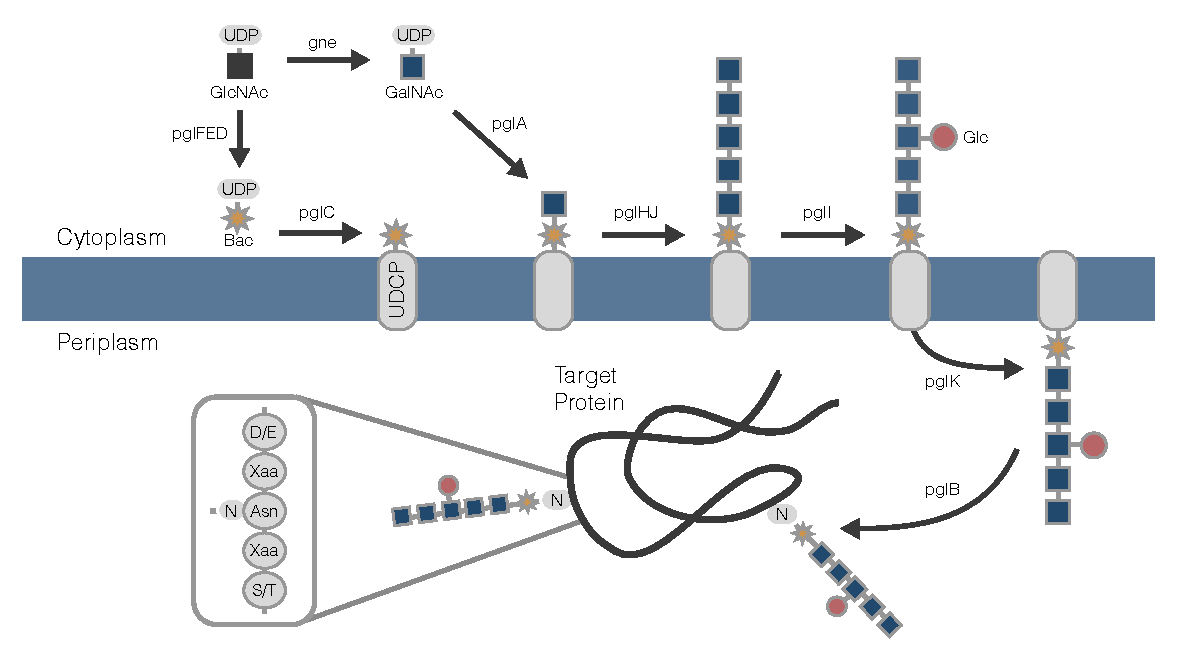
\includegraphics[width=\textwidth]{./figures/fig1-glyco-Ecoli.pdf}
\caption{Glycosylation pathway in \textit{C. jejuni} and \textit{E. coli}. Glycan assembly, facilitated by \textit{pgl} locus enzymes, takes place on a lipid carrier, undecaprenyl pyrophosphate (UDCP), from cytoplasmic pools of nucleotide-activated sugars N-acetylglucosamine (GlcNAc), N-acetylgalactosamine (GalNAc), and glucose (Glc). The glycan is then flipped onto the periplasmic side of the inner membrane, where it is transferred to an asparagine residue on a glycoprotein acceptor motif.}
\label{fig-glyco-Ecoli}
\end{figure}

% Figure 2 - optimization workflow

\clearpage

\begin{figure}\centering
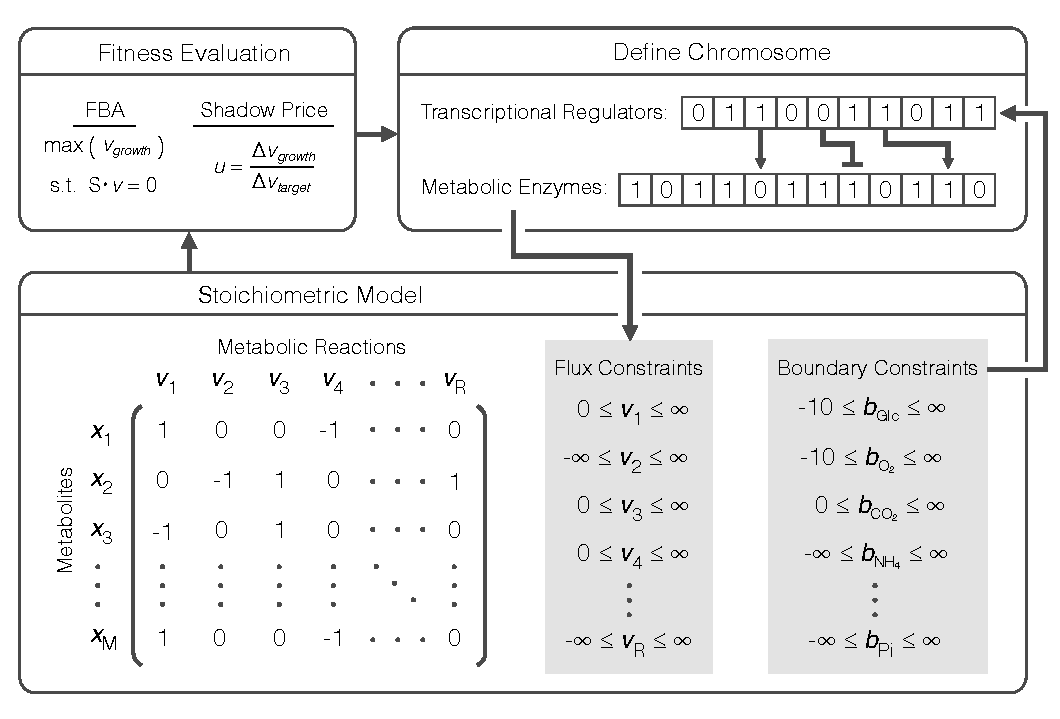
\includegraphics[width=\textwidth]{./figures/fig2-workflow.pdf}
\caption{Heuristic optimization approach used to identify strains coupling growth to glycan production. The chromosome is defined as two separate binary arrays, one defining the state of metabolic enzyme expression and another defining the state of transcriptional regulator activation. Gene repression and knockouts are designated by zeros. Nutrient conditions define the boundary constraints within the stoichiometric model which in turn affect the state of the metabolic enzyme chromosome. Gene repression and knockouts determine the constraints placed on fluxes in the stoichiometric model. Nutrients are mapped to the state of transcriptional regulators and genes are mapped to the state of flux constraints using Boolean rules as defined in \cite{2004-covert-reed-herrgard-palsson-Nat,2007-feist-reed-hatzimanikatis-palsson-MolSysBio}. FBA is used to maximize growth rate under the constraints imposed by the mutant strain and transcriptional regulation and the fitness objective is calculated. Here, we use shadow price. The strain is accepted or rejected based on the change in fitness and a Boltzmann criterion. New mutant strains are randomly generated from accepted ones. The search continues until a positive shadow price is achieved.}
\label{fig-workflow-heuristic}
\end{figure}

% Figure 3 - knockout strain flux analysis

\clearpage

\begin{figure}\centering
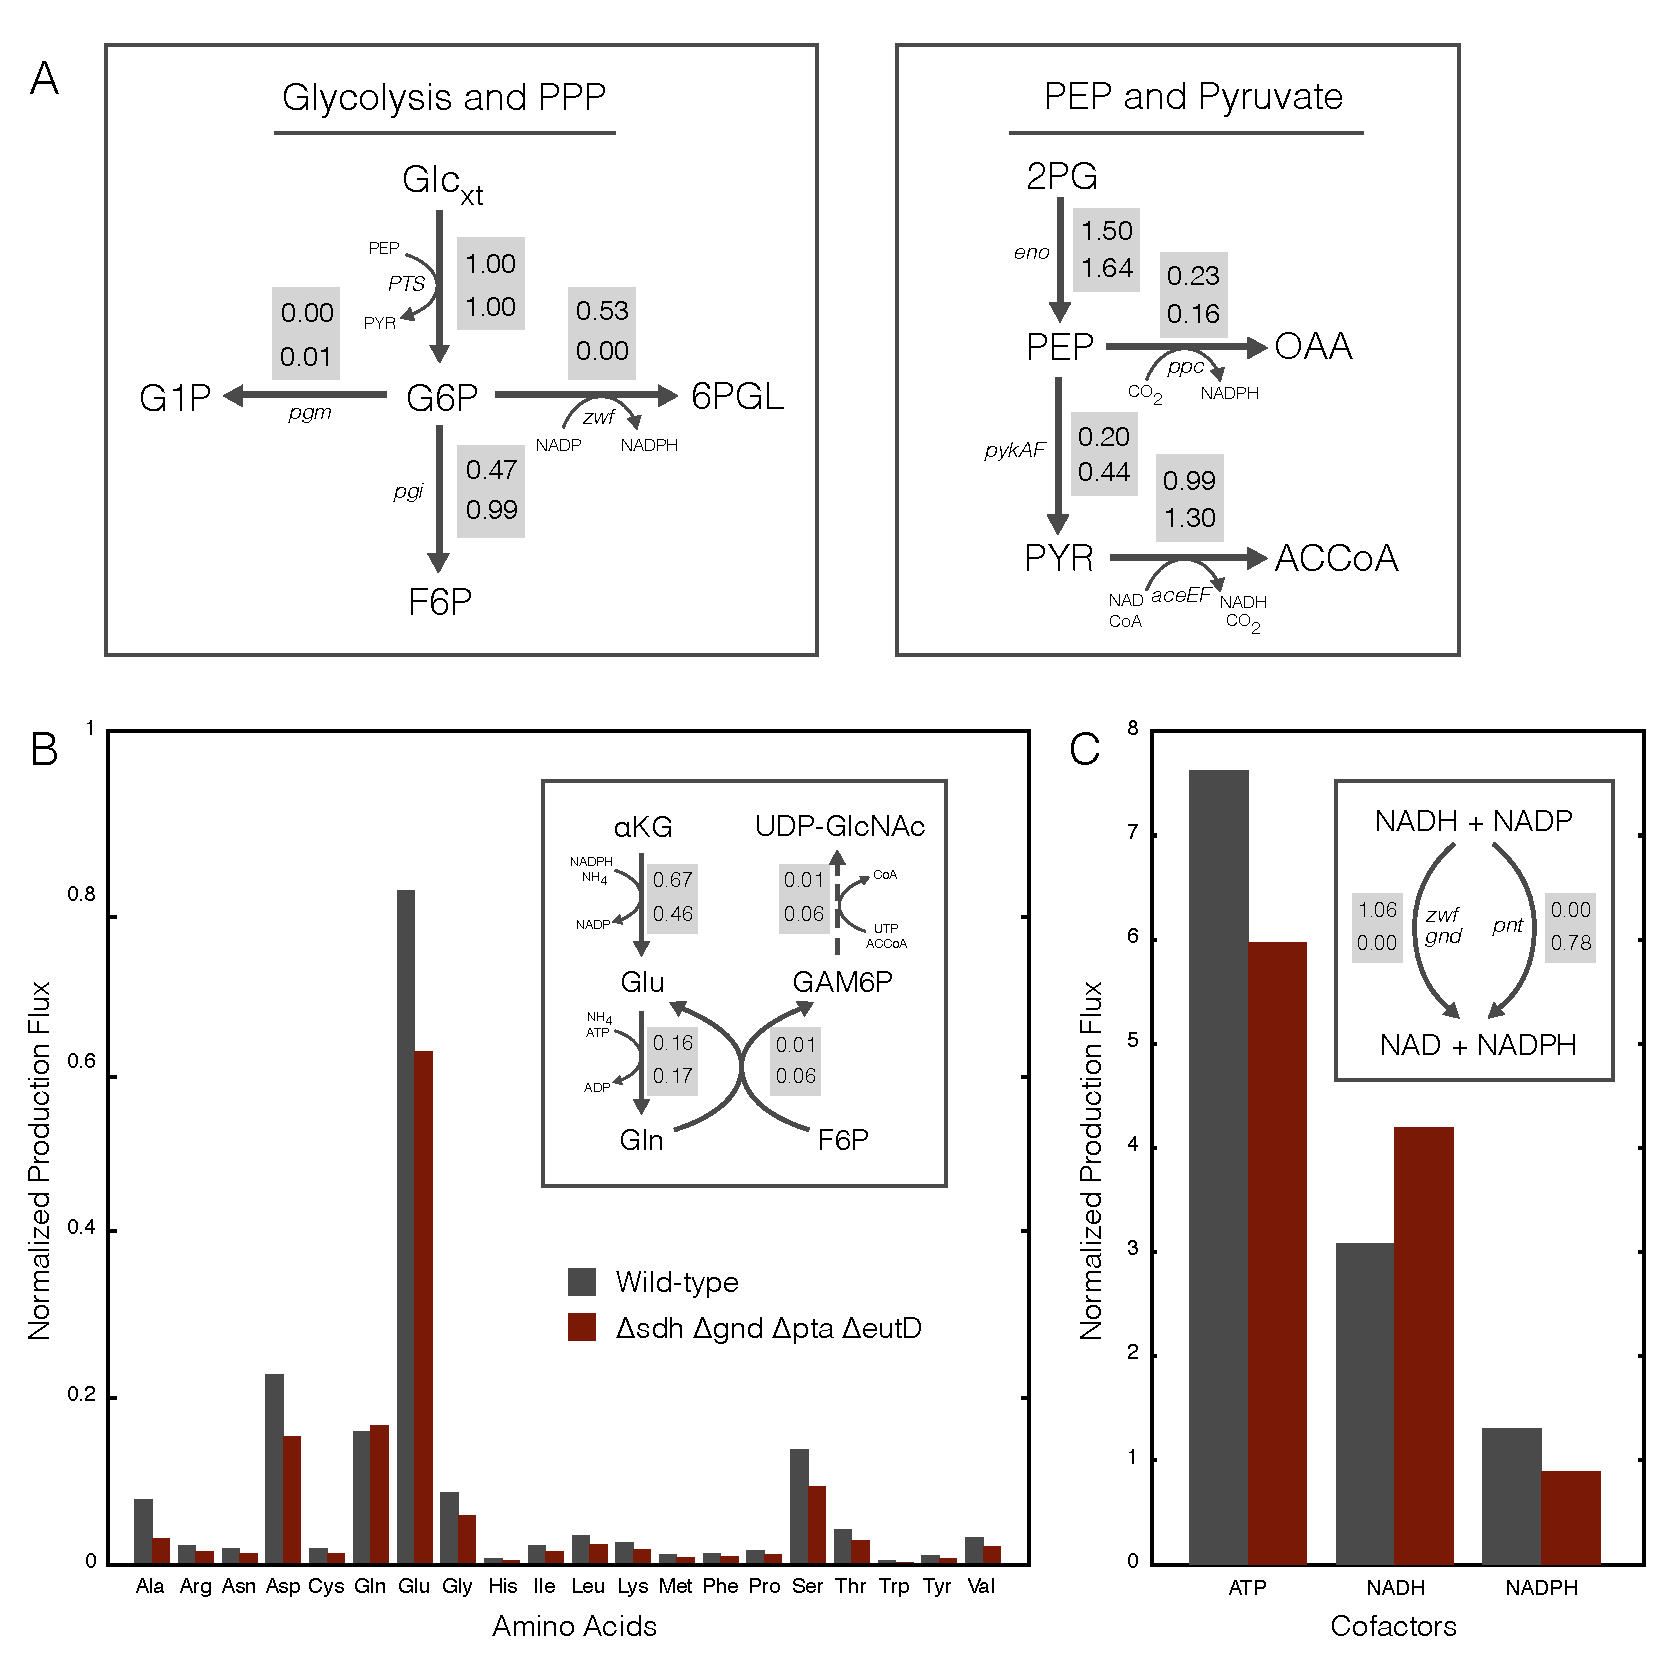
\includegraphics[width=\textwidth]{./figures/fig3-flux-compare.pdf}
\caption{Comparison of fluxes between the wild-type case and glycan-producing strain of type EcGM1 as calculated by FBA. \textbf{(A)} Fluxes through key nodes of metabolism. Top fluxes correspond to the wild-type case, bottom fluxes are for strain EcGM1. Fluxes are normalized by the glucose uptake rate. \textbf{(B)} Total flux into each amino acid, normalized to glucose uptake rate. Inset shows fluxes associated with glutamate and glutamine synthesis along with the pathway to glycan precursor UDP-GlcNAc. The dotted arrow represents a lumped pathway of multiple enzymes leading to the glycan precursor. \textbf{(C)} Total flux into selected cofactors, normalized to glucose uptake rate. Inset shows the primary modes of NADPH production in each strain. Abbreviations: Pentose phosphate pathway, PPP; Extracellular glucose, Glc$_{xt}$; Glucose-6-phosphate, G6P; Fructose 6-phosphate, F6P; 6-phospho D-glucono-1,5-lactone, 6PGL; Glucose 1-phosphate, G1P; Glycerate 2-phosphate, 2PG; Phosphoenolpyruvate, PEP; Pyruvate, PYR; Oxaloacetate, OAA; Acetyl-CoA, ACCoA; 2-Oxoglutarate, $\alpha$KG; Glucosamine 6-phosphate, GAMP6P; UDP-N-acetyl-D-glucosamine, UDP-GlcNAc.
}
\label{fig-KO-flux-analysis}
\end{figure}

% Figure 4 - glycan FACS experiments

\clearpage

\begin{figure}\centering
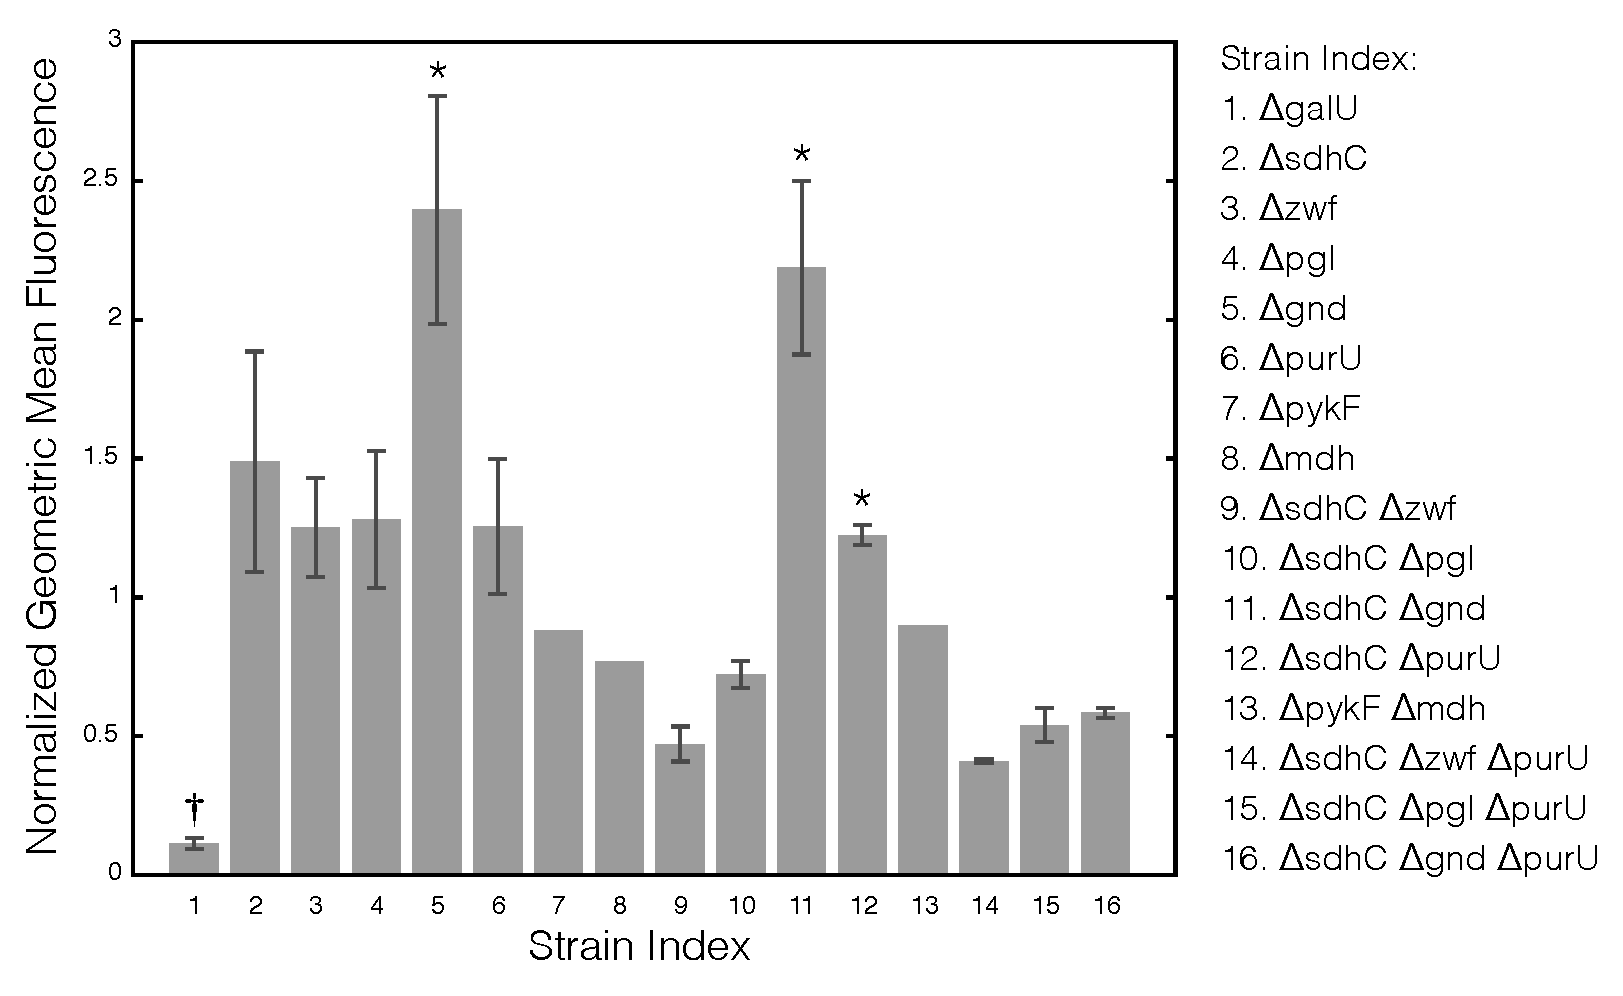
\includegraphics[width=1.0\textwidth]{./figures/fig4-glycan-FACS.pdf}
\caption{Geometric mean fluorescence, normalized to the wild-type value, from gene knockout strains appearing in growth-coupled strains identified by the constraint-based model. $\dagger$ indicates a strain predicted to eliminate glycan flux. Stars indicate statistically significant increases in fluorescences according to a t-test ($p<0.05$). Error bars indicate the average of at least three replicates.}
\label{fig-glycan-FACS}
\end{figure}

% Figure 5 - western blot analysis

\clearpage

\begin{figure}\centering
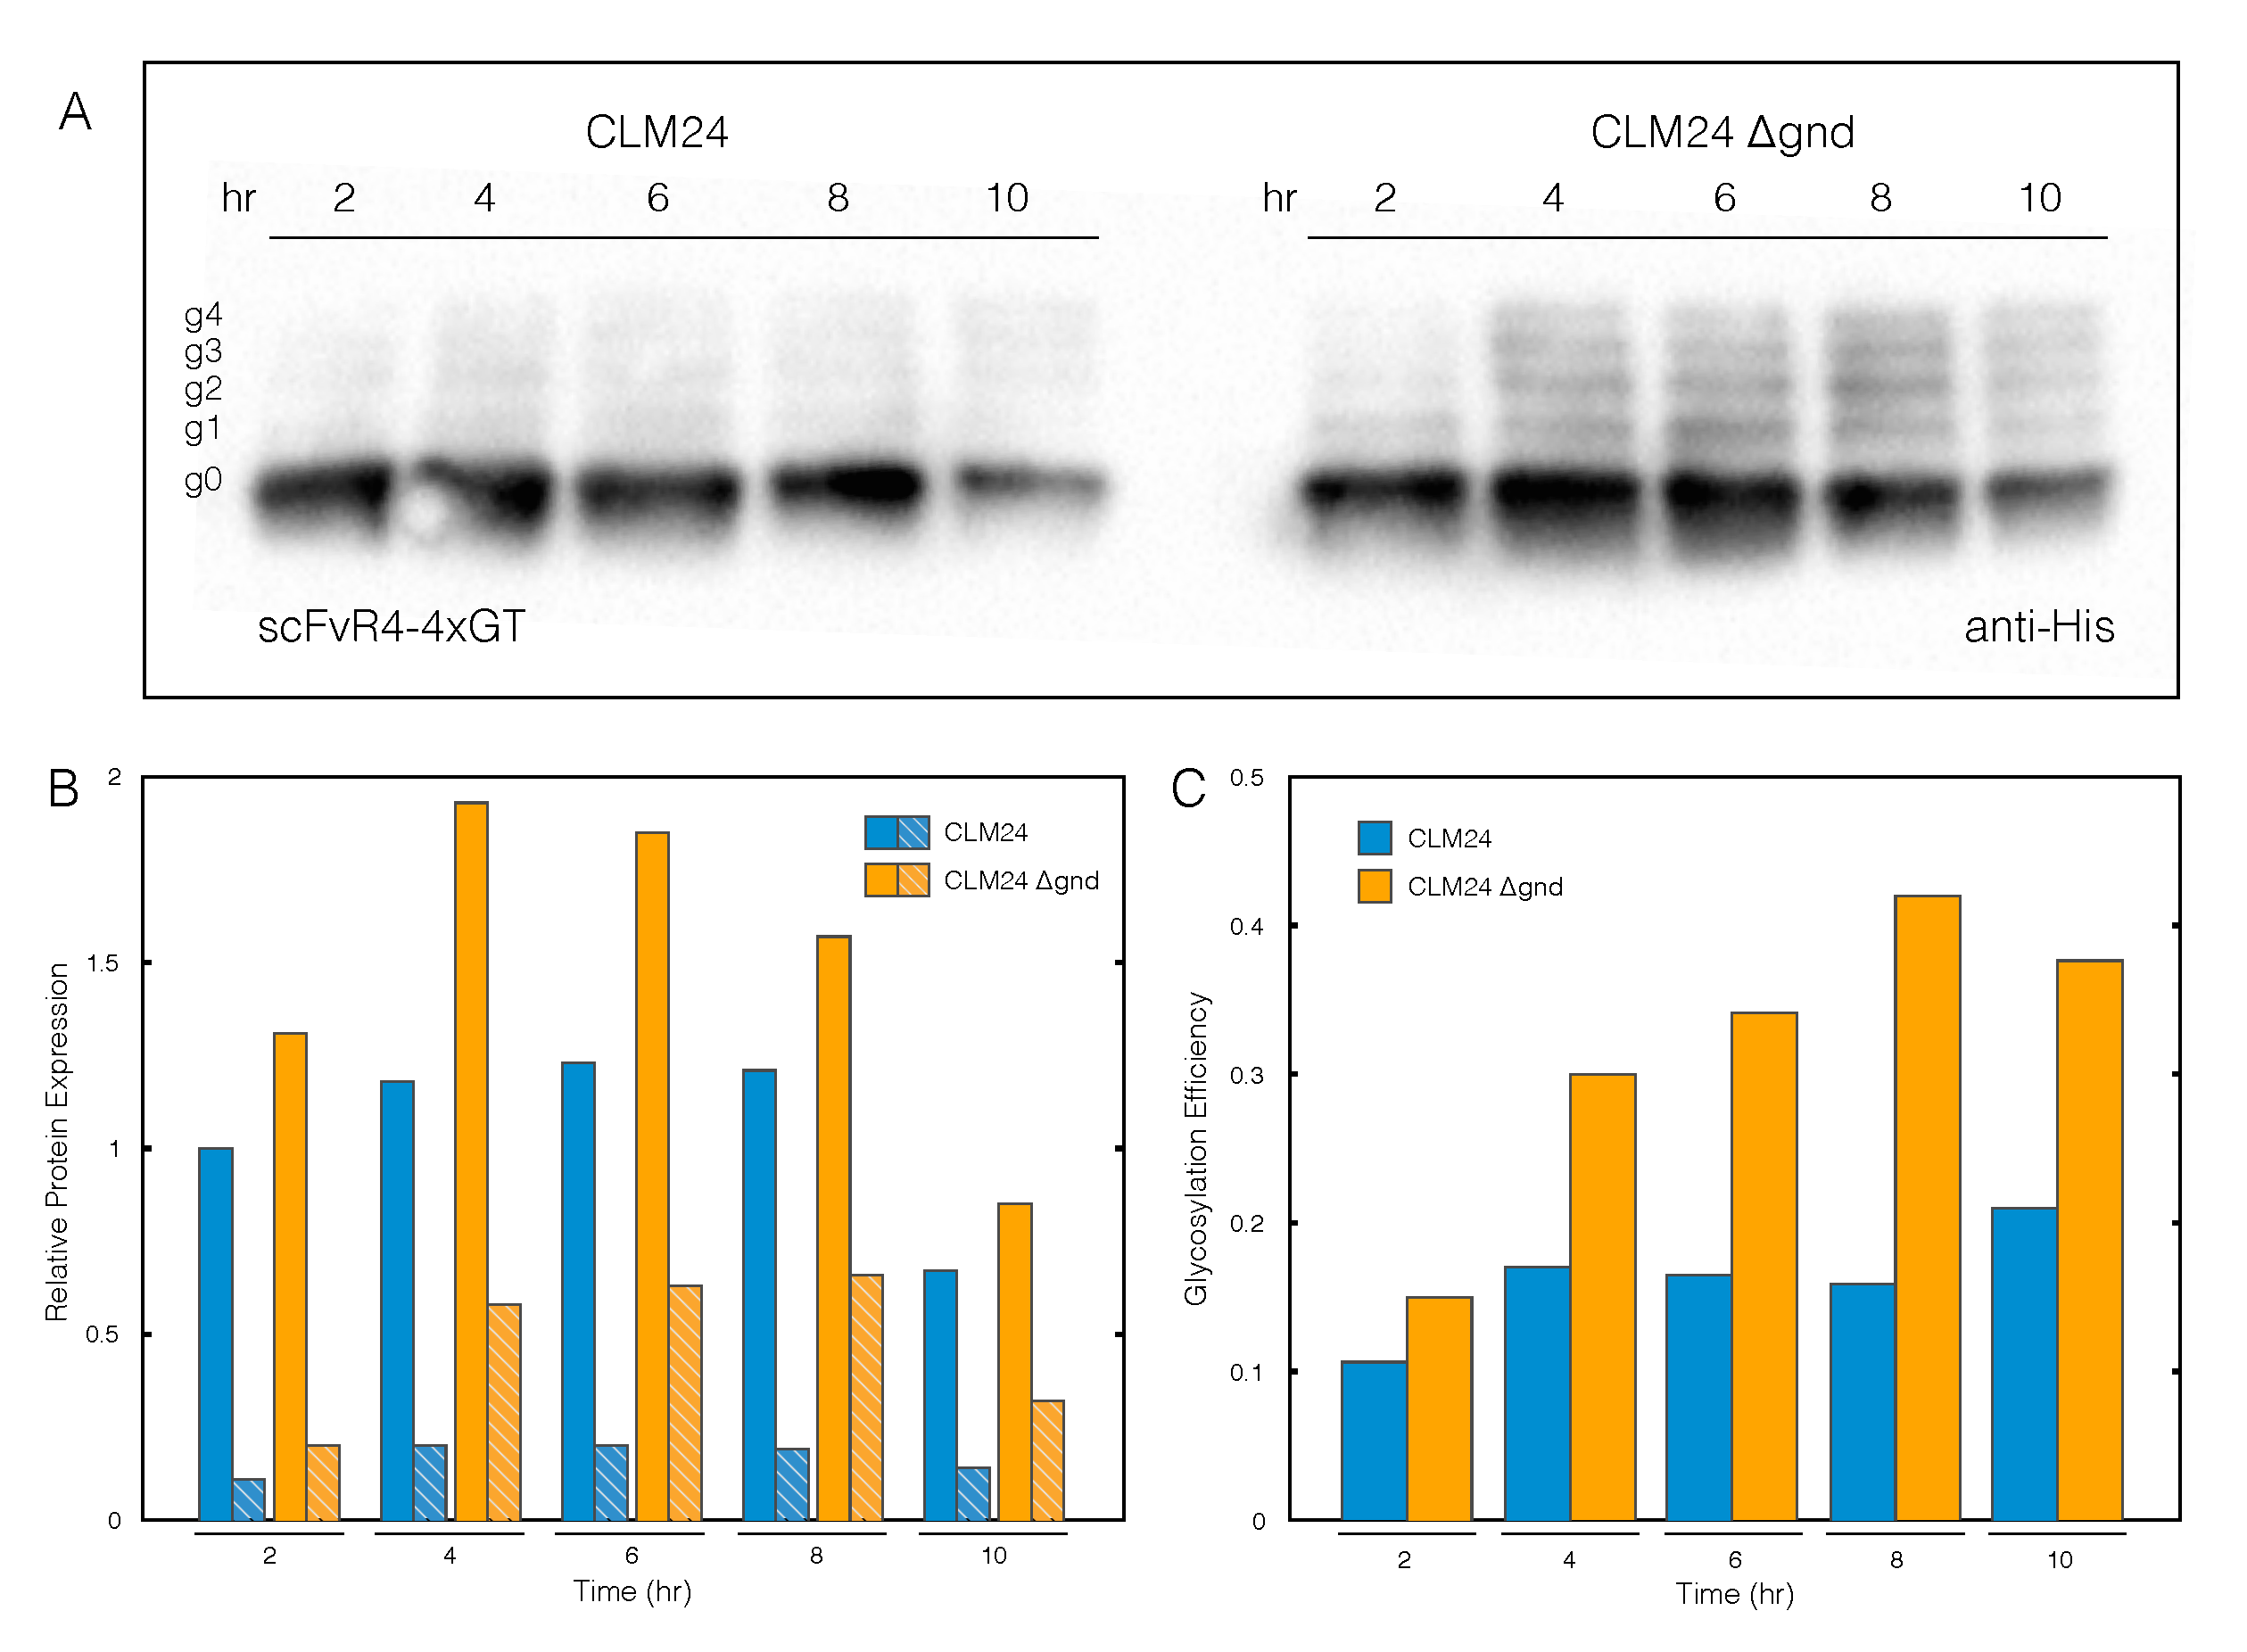
\includegraphics[width=1.0\textwidth]{./figures/fig5-western-gnd.pdf}
\caption{Western blot analysis of glycosylation efficiency in \textit{gnd} mutant. scFvR4 protein expression was induced during exponential growth phase. Time points indicate time after induction. \textit{(A)} Relative protein expression over time. Striped bars indicate the portion of glycosylated protein. \textit{(B)} Glycosylation efficiencies for each strain over time. Blot intensities were determined using image analysis software called ImageJ.}
\label{fig-western-gnd}
\end{figure}


%%%%%%%%%%%%%%%%%%%%%%%%%%%%%%%%%%%%%%%%%%%%%%%%%%%%%%%%%%%%%%%%%%%%%
% TABLES
%%%%%%%%%%%%%%%%%%%%%%%%%%%%%%%%%%%%%%%%%%%%%%%%%%%%%%%%%%%%%%%%%%%%%

% Table 1 - reactions added to model

\clearpage

\begin{table}
\centering
\caption{Reactions added to the \textit{E. coli} model iAF1260 \cite{2007-feist-reed-hatzimanikatis-palsson-MolSysBio} for biosynthesis of \textit{C. jejuni} glycan. Species localized to the periplasm are denoted by (p), all others are cytoplasmic. Abbreviations: UDP-N-Acetyl-D-Glucosamine, UDP-GlcNAc; UDP-N-Acetyl-D-Galactosamine, UDP-GalNAc; UDP-2-acetamido-2,6-dideoxy-$\alpha$-D-xylo-4-hexulose, KetoBac; L-Glutamate, Glu; UDP-N-Acetylbacillosamine, AminoBac; $\alpha$-ketoglutarate, $\alpha$KG; Acetyl-CoA, ACCoA; UDP-N,N'-diacetylbacillosamine, uBac; Coenzyme A, CoA; Undecaprenyl phosphate, Udcpp; \textit{C. jejuni} glycan intermediates, UdcCjGlycan1, UdcCjGlycan6; Uridine monophosphate, UMP; Uridine diphosphate, UDP; UDP-Glucose, UDP-Glc; Lipid-linked \textit{C. jejuni} glycan, UdcCjGlycan; Acceptor protein, AcceptorProt; GlycoProt, Glycoprotein; Undecaprenyl diphosphate, Udcpdp.}
\resizebox{\textwidth}{!}{
\begin{tabular}{llll}
\hline
Gene & Enzyme Name & Reaction & Reference \\
\hline
gne & UDP-GlcNAc epimerase & UDP-GlcNAc $\rightarrow$ UDP-GalNAc & \cite{2005-bernatchez-wakarchuk-JBC} \\
pglF & UDP-GlcNAc dehydratase & UDP-GlcNAc $\rightarrow$ KetoBac + H$_2$O & \cite{2006-schoenhofen-logan-JBC} \\
pglE & Aminotransferase & KetoBac + Glu $\leftrightarrow$ AminoBac + $\alpha$KG & \cite{2006-schoenhofen-logan-JBC} \\ % UDP-4-keto-6-deoxy-GlcNAc aminotransferase
pglD & Acetyltransferase & AminoBac + ACCoA $\rightarrow$ uBac + CoA + H$^+$ & \cite{2006-olivier-imperiali-Biochem} \\
pglC & Bacillosamine transferase & Udcpp + uBac $\rightarrow$ UdcCjGlycan1 + UMP & \cite{2006-glover-imperiali-Biochem} \\
pglAHJ & GalNAc transferases & UdcCjGlycan1 + 5*UDP-GalNAc $\rightarrow$ UdcCjGlycan6 + 5*UDP + 5*H$^+$ & \cite{2005-glover-imperiali-PNAS} \\
pglI & Glucosyl transferase & UdcCjGlycan6 + UDP-Glc $\rightarrow$ UdcCjGlycan + UDP + H$^+$ & \cite{2006-kelly-szymanski-JBact} \\
pglK & ATP-driven flippase & UdcCjGlycan + ATP + H$_2$O $\rightarrow$ UdcCjGlycan(p) + ADP + H$^+$ + Pi & \cite{2006-kelly-szymanski-JBact} \\
pglB & Oligosyltransferase & UdcCjGlycan(p) + AcceptorProt(p) $\rightarrow$ GlycoProt + Udcpdp(p) & \cite{2005-linton-aebi-wren-MolMicrob} \\
\hline
\end{tabular}
}
\label{tbl-pathway-glycan}
\end{table}

% Table 2 - growth-coupled knockout strains

\clearpage

\begin{table}
\centering
\caption{Growth-coupled strains producing \textit{C. jejuni} glycan identified by FBA and heuristic optimization using single carbon substrate. Knockouts listing multiple genes indicate that knockout of any one of those genes produces the same phenotype in the model. Abbreviations: D-Glucose, Glc; \textit{E. coli} glycosylating mutant, EcGM}
\resizebox{\textwidth}{!}{
\begin{tabular}{llllll}
\hline
Strain &  &  & Growth Rate & Glycan Flux & Yield \\
Name & Substrate & Genotype & (/hr) & (mmol/gDW/hr) & (mmol/gDW) \\
\hline 
EcGM1 & Glc & $\Delta$sdh $\Delta$(zwf/pgl/gnd) $\Delta$pta $\Delta$eutD & 0.53 & 0.098 & 0.185 \\
%EcGM2$^\dagger$ & Glc & $\Delta$sdh $\Delta$(zwf/pgl/gnd) $\Delta$purU $\Delta$xdh/allABC $\Delta$pta $\Delta$eutD & 0.58 & 0.055 & 0.095 \\
EcGM2 & Glc & $\Delta$sdh $\Delta$(zwf/pgl/gnd) $\Delta$pykAF $\Delta$mdh & 0.64 & 0.016 & 0.025 \\
EcGM3 & Glc & $\Delta$sdh $\Delta$(zwf/pgl/gnd) & 0.65 & 0.012 & 0.018  \\
%EcGM5$^\dagger$ & Glc & $\Delta$sdh $\Delta$(zwf/pgl/gnd) $\Delta$purU $\Delta$xdh/allABC & 0.65 & 0.007 & 0.011 \\
\hline
%  &  & $\dagger$ Strains without transcription factor regulation &  &   \\
\end{tabular}
}
\label{tbl-KO-strains}
\end{table}

\end{document}
